\documentclass[a4paper,14pt]{extreport} % Основной класс документа — отчёт, ГОСТ-совместимый, 14 pt шрифт

\usepackage{bsuir2025}                  % Подключаем наш собственный стиль оформления

\begin{document}

% -----------------------------------------------------------------------------
% ТИТУЛЬНЫЕ ЛИСТЫ
% -----------------------------------------------------------------------------
\clearpage
\thispagestyle{empty}            % Без номера страницы
% title.tex
\begin{center}
  Министерство образования Республики Беларусь \\
  \bigskip
  Учреждение образования \\
  "<БЕЛОРУССКИЙ ГОСУДАРСТВЕННЫЙ УНИВЕРСИТЕТ ИНФОРМАТИКИ И РАДИОЭЛЕКТРОНИКИ"> \\
  \bigskip \bigskip
  Факультет компьютерных сетей и систем \\
  Кафедра электронных вычислительных средств \\
  \bigskip \bigskip \bigskip \bigskip \bigskip \bigskip \bigskip \bigskip \bigskip \bigskip \bigskip \bigskip
  Отчет по лабораторной работе № 1 \\
  \bf{"<Тема лабораторной работы">}\normalfont \\
  \bigskip \bigskip \bigskip \bigskip \bigskip \bigskip \bigskip \bigskip \bigskip \bigskip \bigskip \bigskip
  \begin{table}[ht]
    \begin{tabular}{p{7cm} p{1cm} p{7cm}}
        Выполнили студенты гр. X5070X \par XXX X.X. \par XXX X.X.\par XXX X.X.& \hfill & \hspace*{30 mm}Проверил \par \hspace*{29 mm} XXX X.X.
    \end{tabular}
  \end{table}
  \vfill \vfill
  \centerline{Минск 2025}
\end{center}
\newpage
                  % Основной титульный лист

% -----------------------------------------------------------------------------
% ТЕХНИЧЕСКОЕ ЗАДАНИЕ (скан, PDF)
% -----------------------------------------------------------------------------
\clearpage
\thispagestyle{empty}

\includepdf[pages=1, pagecommand={}, fitpaper, offset=0 0]{TZ.pdf} % Вставляем первую страницу ТЗ (PDF)

\clearpage
\thispagestyle{empty} 

\includepdf[pages=2, pagecommand={}, fitpaper, offset=0 0]{TZ.pdf} % Вставляем вторую страницу ТЗ

% -----------------------------------------------------------------------------
% ОСНОВНОЙ ДОКУМЕНТ
% -----------------------------------------------------------------------------

\normalfont                         % Устанавливаем стандартный шрифт
\newpage                            % Устанавливаем новую страницу
\setcounter{page}{4}                % Устанавливаем нумерацию с 4 страницы

% Колонтитулы
\pagestyle{fancy}
\fancyhf{}                          % Очищаем все колонтитулы
\fancyfoot[R]{\thepage}             % Номер страницы справа внизу
\renewcommand{\headrulewidth}{0pt}  % Без линии сверху
\renewcommand{\footrulewidth}{0pt}  % Без линии снизу

% Для "plain"-страниц (например, после \chapter)
\fancypagestyle{plain}{%
  \fancyhf{}
  \fancyfoot[R]{\thepage}
  \renewcommand{\headrulewidth}{0pt}
  \renewcommand{\footrulewidth}{0pt}
}

% Настройки шрифта
\normalfont\fontsize{14pt}{14pt}\selectfont

% -----------------------------------------------------------------------------
% ОГЛАВЛЕНИЕ
% -----------------------------------------------------------------------------
\let\oldtableofcontents=\tableofcontents
\renewcommand{\tableofcontents}{\begingroup\parskip=0pt \oldtableofcontents\endgroup}

\noindent\tableofcontents
\addtocontents{toc}{\protect\thispagestyle{fancy}}  % Устанавливаем стиль fancy в оглавлении

% Разрешаем переносы после оглавления
\hyphenpenalty=50
\tolerance=2000

% -----------------------------------------------------------------------------
% ВКЛЮЧЕНИЕ ОСНОВНЫХ РАЗДЕЛОВ
% (Каждая секция — отдельный .tex-файл)
% -----------------------------------------------------------------------------
%------------------------------------------------------------------------------
% \Introduction
%------------------------------------------------------------------------------
\chapter*{\vspace*{-\baselineskip}\begin{center}ВВЕДЕНИЕ\end{center}\vspace*{-\baselineskip*2}}
\addcontentsline{toc}{chapter}{\hspace*{-1em}Введение}\par

%------------------------------------------------------------------------------
% Text
%------------------------------------------------------------------------------
\hspace*{12.5 mm}Распознавание 

Отчет о проверке на заимствования представлен в приложении А.               % Введение
%------------------------------------------------------------------------------
% \PART 1
%------------------------------------------------------------------------------
\chapter[Глава 1]
{Глава 1}

%------------------------------------------------------------------------------
% \PART 1.1 Text
%------------------------------------------------------------------------------
\section{Раздел 1.1}\par
\hspace*{12.5 mm}В данном курсовом проекте ...

%------------------------------------------------------------------------------
% \PART 1.2 Text
%------------------------------------------------------------------------------
\section{Раздел 1.2}\par
\hspace*{12.5 mm}Технические требования                % Глава 1
%------------------------------------------------------------------------------
% \PART 2
%------------------------------------------------------------------------------
\chapter[Предварительное проеектирование системы]{ПРЕДВАРИТЕЛЬНОЕ ПРОЕКТИРОВАНИЕ СИСТЕМЫ}

%------------------------------------------------------------------------------
% \PART 2.1 Text
%------------------------------------------------------------------------------
\section{Разбиение системы на модули}
\hspace*{12.5 mm}Для обеспечения надёжной работы системы 
фотоаппарата на базе микроконтроллера ESP32-CAM был разбит
на несколько функциональных модулей. 
Каждый модуль отвечает за выполнение определённых задач, что 
упрощает разработку и тестирование устройства. Основные модули 
системы:

    1 Модуль инициализации камеры.
Этот модуль отвечает за конфигурацию и запуск камеры ESP32-CAM. 
В нём задаются параметры камеры, такие как частота тактирования 
(XCLK), разрешение изображения (1024x768 пикселей) и формат 
данных (JPEG). Также модуль управляет буферами кадров для 
хранения изображений, полученных с камеры.

    2 Модуль управления веб-сервером.
Данный блок реализует веб-сервер на основе ESP32s, который предоставляет 
пользователю доступ к функционалу устройства через веб-браузер. 
Он обрабатывает запросы на:
    
    - Отображение видео потока с камеры в режиме реального времени.

    - Съёмку фотографий и сохранение их на SD-карту.

    - Возврат страницы с подтверждением успешного выполнения операции.

    3 Модуль захвата и сохранения изображений.
После получения команды от веб-сервера этот модуль захватывает 
кадр с камеры, конвертирует его в JPEG и сохраняет на SD-карту. 
Каждое изображение получает уникальное имя, основанное на 
текущем времени, чтобы избежать перезаписи существующих файлов.

    4 Модуль управления Wi-Fi.
Этот модуль настраивает и управляет точкой доступа Wi-Fi, 
создаваемой микроконтроллером ESP32-CAM. Он позволяет пользователю 
подключаться к устройству через беспроводную сеть и 
взаимодействовать с веб-интерфейсом. Для этого задаются 
параметры SSID и пароля для доступа.

    5 Модуль работы с файловой системой.
Данный блок отвечает за работу с файловой системой SD-карты. 
Он инициализирует SD-карту, открывает и закрывает файлы для 
записи, а также проверяет наличие свободного места для 
сохранения изображений.

%------------------------------------------------------------------------------
% \PART 2.2 Text
%------------------------------------------------------------------------------
\section{Разработка структурной схемы устройства}
\hspace*{12.5 mm}Устройство, реализованное в данном курсовом 
проекте, состоит из трёх основных аппаратных блоков:

    1 Модуль камеры OV2640.

    2 Память на основе SD-карты. 

    3 Микроконтроллер ESP32-cam. 
    
    Модуль OV2640 обеспечивает захват изображения с 
последующим преобразованием его в цифровой формат 
для дальнейшей обработки микроконтроллером ESP32-cam.

    Для долговременного хранения 
изображений используется SD-карта на 4Гб, которая отформатирована в 
файловой системе FAT32. Этот формат широко поддерживается и 
позволяет легко работать с большими файлами. В данном проекте 
SD-карта служит для хранения снимков, захваченных камерой, в 
формате JPEG.

    Микроконтроллер ESP32-cam — это основной вычислительный 
блок системы, который управляет работой камеры, обработкой 
изображений, сохранением данных на SD-карту и организацией 
взаимодействия с пользователем через веб-интерфейс.

    Для удобства разработки и упрощения структуры программного 
обеспечения микроконтроллер ESP32-cam разделён на несколько 
модулей, каждый из которых выполняет свои специфические функции.

Схема электрическая структурная представлена в Приложении А.               % Глава 2
%------------------------------------------------------------------------------
% \PART 3
%------------------------------------------------------------------------------
\chapter[Глава 3]
{ГЛАВА 3}

%------------------------------------------------------------------------------
% \PART 3.1 Text
%------------------------------------------------------------------------------
\section{Раздел 3.1}\par
\hspace*{12.5 mm}При 

%------------------------------------------------------------------------------
% \PART 3.2
%------------------------------------------------------------------------------
\section{Раздел 3.2}\par
\hspace*{12.5 mm}В 

\bf{3.2.1} \normalfont{Пункт без названия} 

Пример ссылки на изображение и на источник литературы:
% На рисунке~\ref{fig:esp32s} представлена распиновка ESP32S\cite{ESP-S}.

Пример вставки изображения.
% \insertfigure{esp32s}{pic/esp32s.png}{Микроконтроллер ESP32S}{9cm}
               % Глава 3
%------------------------------------------------------------------------------
% \PART 4
%------------------------------------------------------------------------------
\chapter[Разработка IP-блока нейронной сети для распознавания рукописных цифр]
{РАЗРАБОТКА IP-БЛОКА НЕЙРОННОЙ СЕТИ ДЛЯ РАСПОЗНАВАНИЯ РУКОПИСНЫХ ЦИФР}

%------------------------------------------------------------------------------
% \PART 4.1 Text
%------------------------------------------------------------------------------
\section{Представление исходных данных}\par
\hspace*{12.5 mm}В качестве исходных данных используется набор MNIST, 
содержащий 70 тысяч полутоновых изображений размера $28 \times 28$ пикселей, 
представляющих рукописные цифры от 0 до 9~\cite{MNIST}. Данный набор разделен 
на две части:

  – \text{Тренировочная выборка} – 60 тысяч изображений, используемых для 
обучения модели.

  – \text{Тестовая выборка} – 10 тысяч изображений, предназначенных для 
проверки качества работы обученной нейросети.

    Пример данных из базы MNIST представлен на рисунке~\ref{fig:mnist}.

\insertfigure{mnist}{pic/MNIST.jpeg}{Пример данных из MNIST}{11.5cm}

Перед подачей в нейросеть изображения проходят предварительную обработку, 
включающую нормализацию значений пикселей. Каждый пиксель исходного изображения
представлен числом в диапазоне от 0 до 255 (градации серого). Для упрощения 
процесса обучения выполняется нормализация данных таким образом, чтобы значение 
каждого пикселя было в диапазоне от $-1$ до $1$, а стандартное отклонение 
($\sigma$) составляло $0.5$. Это позволяет сделать градиентный спуск более 
устойчивым и ускорить процесс сходимости модели. Пример такой обработки 
представлен на рисунке~\ref{fig:norm-img}.

\insertfigure{norm-img}{pic/norm_img.png}{Пример обработанных данных из MNIST}{9cm}

Для аппаратной реализации на FPGA числа представляются в формате с 
фиксированной запятой (Fixed-Point). В отличие от чисел с плавающей запятой 
(Floating-Point), данный формат обеспечивает более эффективное использование 
аппаратных ресурсов, таких как блоки DSP и BRAM.\@

В данной работе используется фиксированное представление с разрядностью $Q6.8$,
где:

  – 6 бит отведены под целую часть числа.

  – 8 бит используются для дробной части.

Таким образом, числа в этом формате могут представлять значения в диапазоне 
$[-32, 31.996]$ с шагом $2^{-8} = 0.00390625$.

При переводе значений из плавающей запятой в фиксированную используется метод 
округления к ближайшему минимальному числу (округление вниз, или Round Down). 
Этот метод позволяет минимизировать ошибки округления и избежать 
систематического смещения, которое может возникать при округлении к ближайшему 
числу.

Такой метод округления позволяет повысить точность вычислений и уменьшить 
накопление ошибок при последовательных операциях, что критично для работы 
нейросети на FPGA.\@

%------------------------------------------------------------------------------
% \PART 4.2 Text
%------------------------------------------------------------------------------
\section{Обучение нейронной сети}
\hspace*{12.5 mm}Обучение нейронной сети LST-1 на основе 60000 тренировочных 
изображений из базы данных MNIST.\@ Для обучения используется фреймворк 
PyTorch.

Из MNIST загружается 60000 тренировочных и 10000 тестовых изображений размером 
\(28 \times 28\) пикселей в градациях серого. Из тренировочного набора 
выделяется 1000 изображений для валидации, оставшиеся 59000 используются для 
непосредственного обучения модели. 

Нормализация изображений осуществляется в соответствии с описанными ранее 
требованиями.

\small
\fontsize{12pt}{12pt}\selectfont
\begin{verbatim}
    transform = transforms.Compose([
        transforms.ToTensor(),
        transforms.Normalize((0.5,), (0.5,))
    ])
\end{verbatim}
\normalsize
\fontsize{14pt}{14pt}\selectfont

Модель L2DST состоит из двух линейных слоев LazyLinear с функцией активации 
tanh и полносвязный слой Linear с функцией активации softmax для классификации. 

В качестве метрики, для оценки обучаемости нейронной сети используется функция 
потерь кросс-энтропии – {Negative Log-Likelihood Loss (NLLLoss)}.

Оптимизатор {Adam} с параметром скорости обучения \(1.5 \times 10^{-3}\) и 
шаговым снижением {StepLR} (с понижением на 3\% каждые 10 эпох).
 
\small
\fontsize{12pt}{12pt}\selectfont
\begin{verbatim}
    class L2DST(nn.Module):
    def __init__(self, ffn_num_hiddens, ffn_num_outputs):
        super().__init__()
        self.dense1 = nn.LazyLinear(ffn_num_hiddens)
        self.dense2 = nn.LazyLinear(ffn_num_outputs)

    def forward(self, X):
        out = torch.nn.functional.tanh(self.dense1(X))
        out1 = torch.transpose(out, -1, -2)
        out = torch.nn.functional.tanh(self.dense2(out1))
        out = torch.transpose(out, -2, -1)
        return out

criterion = nn.NLLLoss() 
optimizer = optim.Adam(model.parameters(), lr=15e-4, weight_decay=0e-5)
scheduler = lr_scheduler.StepLR(optimizer, step_size=10, gamma=0.97, 
                                                         verbose=False)
\end{verbatim}
\normalsize
\fontsize{14pt}{14pt}\selectfont


Обучение проводится на 370 эпохах, при этом на каждой эпохе вычисляется функция
потерь {NLLLoss}. На рисунке~\ref{fig:loss} показан график функции потерь.

\insertfigure{loss}{pic/loss.png}{Графики функции потерь на обучающем и тестовом наборе}{9cm}

После завершения каждой эпохи вычисляются средние ошибки на тренировочном и 
валидационном наборах данных.  

Python описание процесса обучения нейронной сети прямого распространения 
приведено в приложении Д.

%------------------------------------------------------------------------------
% \PART 4.3 Text
%------------------------------------------------------------------------------
\section{Программная реализация эталонной модели нейронной сети на языке Python}
\hspace*{12.5 mm}Программная реализация нейронной сети выполняется с 
использованием языка Python и специализированных библиотек машинного обучения.  
В качестве эталонной модели реализуется нейронная сеть на основе библиотеки 
{fixpoint}, позволяющая провести сравнение точности вычислений при 
использовании чисел с фиксированной запятой и чисел с плавающей запятой.

Эталонная модель представляет собой нейросеть с двумя скрытыми слоями и 
активационной функцией {tanh}.  

Входные изображения размером \(28 \times 28\) проходят последовательную 
обработку:

  – Первый слой выполняет линейное преобразование входных данных с весами и 
смещением, после чего применяется функция активации тангенс.
    
  – Второй слой аналогично выполняет линейное преобразование, используя 
параметры весов и смещений, после чего применяется функция активации тангенс.
    
  – Выходной слой выполняет классификацию, вычисляя вероятности классов с 
помощью softmax.

Для проверки корректности работы алгоритма в числах с фиксированной запятой 
разрабатывается программная эмуляция аппаратного вычислителя. Эмуляция 
реализуется с использованием классов:

  1 {MAC} – блок умножения и аккумуляции с фиксированной точностью.
    
  2 {MEM} – память для хранения весов и промежуточных значений.
    
  3 {TANH} – реализация функции гиперболического тангенса в фиксированной 
точности.

Обработка входных данных в модели с фиксированной запятой включает следующие 
этапы:

  1 Загрузка изображения из базы данных MNIST в память.

  2 Преобразование входных данных согласно формату Q6.8.
    
  3 Выполнение первого преобразования и применение функции тангенс.

  4 Обработка данных во втором слое с аналогичной активацией.

  5 Вычисление выходных значений нейросети и применение softmax.

Сравнение выходных значений между моделью с фиксированной точностью и моделью с
плавающей точкой представлено на рисунке~\ref{fig:dif}.  

\insertfigure{dif}{pic/difpng.png}{Сравнение результатов вычислений}{13.5cm}

Графический анализ разности значений в обработке одного и того же изображения 
позволяет оценить влияние округлений и возможные потери точности.

Разработанная эталонная модель на Python позволяет проверить корректность 
вычислений перед аппаратной реализацией, а также провести тестирование 
точности чисел с фиксированной запятой.

Python описание нейронной сети с использованием библиотеки fixpoint приведено в
приложении Д.

%------------------------------------------------------------------------------
% \PART 4.4 Text
%------------------------------------------------------------------------------
\section{Разработка операционной части нейронной сети}
\hspace*{12.5 mm}Нейронная сеть есть объединение управляющего и операционного
автоматов, что показано на рисунке~\ref{fig:operat}. 

\insertfigure{operat}{pic/operational.png}{Представление нейронной сети в виде управляющего и операционного автоматов}{16cm}

Элементарное действие, выполняемое в операционном автомате, называется 
микрооперацией. Пусть множество микроопераций, выполняемых под воздействием 
сигналов управляющего автомата, обозначается как \( Y = y_1, \dots, y_N\).  

Для выполнения микрооперации \( y_i \) (\( i = 1, \dots, N \)) необходимо 
появление соответствующего управляющего сигнала, принимающего значение единицы. 
Если в операционном автомате одновременно выполняется несколько микроопераций, 
они образуют микрокоманду.  

Множество микрокоманд в совокупности с логическими условиями 
\(X = x_1, \dots, x_N \), определяющими последовательность их выполнения, 
составляют микропрограмму. Логические условия соответствуют осведомительным 
сигналам, которые формируются в операционном автомате.

IP-блок нейронной сети должен быть спроектирован как независимый компонент 
системы, обеспечивающий модульность и возможность интеграции в различные 
вычислительные среды. Для этого необходимо, чтобы блок обладал четко 
определенным и простым интерфейсом, что позволит эффективно взаимодействовать 
с другими компонентами системы.

Интерфейс IP-блока должен обеспечивать передачу входных данных, управление 
процессом вычислений и выдачу результатов. Важно, чтобы структура 
взаимодействия соответствовала требованиям к гибкости и масштабируемости 
системы. На рисунке~\ref{fig:interface} представлен требуемый вид интерфейса 
IP-блока, демонстрирующий основные входные и выходные сигналы, а также 
механизмы управления вычислительным процессом.

\insertfigure{interface}{pic/interface.png}{Интерфейс IP-блока нейронной сети}{6cm}

%------------------------------------------------------------------------------
% \PART 4.5 Text
%------------------------------------------------------------------------------
\section{Проектирование функциональной схемы нейронной сети}
\hspace*{12.5 mm}При разработке IP-блока нейронной сети необходимо определить 
его функциональную структуру, обеспечивающую корректное выполнение вычислений, 
взаимодействие с внешними компонентами системы и эффективное управление 
процессом обработки данных.

Функциональная схема IP-блока должна описывать основные модули и их 
взаимодействие, включая блоки обработки входных данных, вычислительное ядро 
нейронной сети, управляющий модуль и интерфейсы для связи с внешней средой. 
Важно учитывать требования к производительности, ресурсоемкости и 
масштабируемости, чтобы обеспечить возможность интеграции IP-блока в различные 
аппаратные платформы.

Также на функциональной схеме показаны микрооперации и логические условия. 
Данная нейронная сеть состоит из нескольких основных блоков. Существует два 
типа блоков обработки пикселя, которые отличаются количеством блоков памяти,
которые должны обрабатываться мультиплексором и поступать в качестве входных 
данных на умножитель.

После вычисления полносвязного слоя для конкретной строки или столбца данные 
поступают в регистр обработки, состоящий из 28 чисел разрядностью 13 бит. 
Затем данные из этого регистра последовательно поступают в регистр данных 
тангенса, из которого они отправляются в блок аппроксимации тангенса 
гиперболического.

Также используются два пяти разрядных и один десяти разрядный счетчики, которые
используются для генерации адреса в память весов и в память изображения.

Блок функции активации softmax реализован на принципе сравнения всех десяти 
входных классов и выбора наибольшего значения, что будет соответствует наиболее
вероятному значению. В результате на выход поступает индекс максимального 
элемента.

Для управления работой и генерирования микроопераций на основе логических 
условий используется микропрограммный автомат.

Электрическая функциональная схема IP-блока нейронной сети прямого 
распространения приведена в приложении Е.

%------------------------------------------------------------------------------
% \PART 4.6 Text
%------------------------------------------------------------------------------
\section{Построение микропрограммы работы нейронной сети}
\hspace*{12.5 mm}На данном этапе проектирования создается микропрограмма, 
определяющая последовательность выполнения операций внутри IP-блока нейронной 
сети. Она описывает порядок обработки входных данных, передачу информации между 
модулями и выполнение вычислений.

Микропрограмма строится на основе дискретных состояний, в которых выполняются 
конкретные микрооперации. Каждое состояние характеризуется активными 
управляющими сигналами, обеспечивающими выполнение определенной части 
вычислений.

Основные этапы работы микропрограммы включают:

  1 Загрузку изображения в память – входные данные загружаются в буфер 
оперативной памяти, откуда они будут переданы в вычислительные блоки.

  2 Выполнение операций LST-преобразования – производится начальная обработка 
изображения, включающая нормализацию и предварительное выделение признаков.

  3 Передача данных в полносвязный слой – результаты преобразования передаются 
в полносвязный слой нейросети для дальнейшей обработки.

  4 Выполнение финальной классификации – производится анализ данных нейросетью
и определение класса входного изображения.

  5 Отправка данных в систему обработки – результаты классификации передаются
в систему для последующего использования.

Микропрограмма работы нейронной сети по распознаванию рукописных цифр 
представлена в Приложении Ж. Данная схема отображают основные микрооперации и 
логические условия.

%------------------------------------------------------------------------------
% \PART 4.7 Text
%------------------------------------------------------------------------------
\section{Проектирование управляющей части}
\hspace*{12.5 mm}Проектирование управляющей части вычислительного устройства 
осуществляется методом структурирования конечных состояний системы на основе 
синхронных схем – каноническим методом структурного синтеза микропрограммного 
автомата (МПА). На этапе структурного синтеза принято представлять МПА в виде 
двух частей: памяти и комбинационной схемы, что представлено на 
рисунке~\ref{fig:cnn-pic}.

Память автомата состоит из заранее выбранных элементов памяти, обеспечивающих 
хранение информации о текущем состоянии устройства. В качестве элементов памяти 
используются триггеры, которые позволяют надежно фиксировать и изменять 
состояние системы.  

Количество элементов памяти, необходимых для хранения состояний автомата, 
определяется по следующей формуле:

\begin{equation}
    N = \log_{2}{M},
\end{equation}

\noindentгде $M$ – число состояний микропрограммного автомата.  

Однако в практических реализациях часто применяется кодирование состояний с 
использованием кода Грея. Код Грея представляет собой двоичную систему 
кодирования, в которой любые два последовательных числа отличаются изменением 
только одного бита\cite{Tokheim2003}. Это позволяет уменьшить количество 
переключений триггеров при переходе между состояниями, снижая вероятность 
ошибок, возникающих из-за временных несовпадений сигналов.  

\insertfigure{cnn-pic}{pic/cnt.png}{Представление управляющей части нейронной сети в виде композиции памяти и комбинационной схемы}{10cm}

Дополнительно, в разработке автоматов управления применяется стратегия, при 
которой старший бит кодового слова указывает на нахождение автомата в состоянии
ожидания. Это состояние используется для инициализации системы, сброса 
счетчиков и минимизации нежелательных переходов. Применение старшего 
бита в качестве указателя на режим ожидания помогает уменьшить влияние гличей 
(glitch) на граф переходов. Гличи – это кратковременные нежелательные изменения
сигнала, возникающие при переключении состояний из-за различий во времени 
распространения сигналов через логические элементы~\cite{Katz1994}. Они могут 
приводить к некорректным переходам в автомате, вызывая ошибки в работе системы.  

В связи с этим, традиционная формула определения числа элементов памяти 
модифицируется следующим образом:

\begin{equation}
    N = \log_{2}{M} + 1 = \log_{2}{11} + 1 = 5,
\end{equation}

\noindentгде $M = 11$ – число состояний микропрограммного автомата.  

Таким образом, каждое состояние автомата описывается представлением из 5 бит, 
что позволяет повысить надежность работы системы, уменьшить количество 
переключений триггеров и снизить вероятность ошибок, связанных с гличами.  

Закодированные состояния автомата представлены в таблице 1.

В соответствии со списком микроопераций (Y) и логических условий (X), а также 
разработанной микропрограммой составим граф-схему алгоритма, которая 
представлена на рисунке~\ref{fig:gs}.

\begin{table*}[ht]
  Таблица 1 – Кодирование состояний автомата\par
  \renewcommand{\arraystretch}{1.2}
  \begin{tabularx}{\textwidth}{|c|>{\centering\arraybackslash}X|}
    \hline
    Состояние & Код Грея (\(T_4T_3T_2T_1T_0\)) \\ \hline
    \(a_0   \)   & 00000                       \\ \hline
    \(a_1   \)   & 10000                       \\ \hline
    \(a_2   \)   & 10001                       \\ \hline
    \(a_3   \)   & 10011                       \\ \hline
    \(a_4   \)   & 10010                       \\ \hline
    \(a_5   \)   & 10110                       \\ \hline
    \(a_6   \)   & 10111                       \\ \hline
    \(a_7   \)   & 10101                       \\ \hline
    \(a_8   \)   & 11101                       \\ \hline
    \(a_9   \)   & 11111                       \\ \hline
    \(a_{10}\)   & 11110                       \\ \hline
  \end{tabularx}
\end{table*}

\insertfigure{gs}{pic/gs.png}{Граф переходов}{16cm}

Важно отметить, что для упрощения понимания и реализации управляющего 
устройства некоторые состояния разбиты на группу из нескольких состояний. В 
соответствии с разработанной граф-схемой алгоритма составлена таблица 2, в 
которой представлены все переходы и их условия.

\begin{table*}[ht]
  Таблица 2 – Таблица переходов граф-схемы алгоритма\par
  \renewcommand{\arraystretch}{1.2}
  \begin{tabularx}{\textwidth}{|c|c|c|c|c|>{\centering\arraybackslash}X|}
    \hline
    h  & $a_m$    & $a_s$    & $X_h$               &                                           & \(Y_t\)                                \\ \hline
    1  & $a_0$    & $a_0$    & $\overline{x_0}$    &  –                                        & –                                      \\ \hline
    2  &          & $a_1$    & $x_0$               & $Y_1$                                     & $y_0, y_1, y_4, y_6, y_7, y_9, y_{10}$ \\ \hline
    3  & $a_1$    & $a_1$    & $\overline{x_1}$    &  –                                        &  –                                     \\ \hline
    4  &          & $a_2$    & $x_1$               &  –                                        &  –                                     \\ \hline
    5  & $a_2$    & $a_3$    &  1                  & $Y_2$                                     & $y_2$                                  \\ \hline
    6  & $a_3$    & $a_4$    &  1                  & $Y_3$                                     & $y_0, y_1, y_3$                        \\ \hline
    7  & $a_4$    & $a_4$    & $\overline{x_2}$    & $Y_4$                                     & $y_6$                                  \\ \hline
    8  &          & $a_5$    & $x_2$               &  –                                        &  –                                     \\ \hline
    9  & $a_5$    & $a_6$    &  1                  & $Y_5$                                     & $y_5$                                  \\ \hline
    10 & $a_6$    & $a_6$    & $x_4$ | $\overline{x_4}x_5$ | $\overline{x_4}\overline{x_5}x_6$ & – | $Y_6$ | $Y_7$  & $y_6, y_7$        \\ \hline
    11 &          & $a_7$    & ${x_2}$             & $Y_8$                                     & $y_8$                                  \\ \hline
    12 & $a_7$    & $a_3$    & $\overline{x_3}$    & $Y_9$                                     & $y_4$                                  \\ \hline
    13 &          & $a_8$    & $x_3$               & $Y_{10}$                                  & $y_{10}$                               \\ \hline
    14 & $a_8$    & $a_9$    &  1                  &  –                                        &   –                                    \\ \hline
    15 & $a_9$    & $a_9$    & $\overline{x_7}$    & $Y_{11}$                                  & $y_{11}$                               \\ \hline
    16 &          & $a_{10}$ & $x_7$               &  –                                        &   –                                    \\ \hline
    17 & $a_{10}$ & $a_0$    &  1                  &  –                                        &   –                                    \\ \hline
  \end{tabularx}
\end{table*}

%------------------------------------------------------------------------------
% \PART 4.8 Text
%------------------------------------------------------------------------------
\section{Построение графа переходов управляющего автомата}

\hspace*{12.5 mm}Граф переходов управляющего автомата позволяет представить 
граф-схему алгоритма в соответствии с условными обозначениями. Граф переходов 
управляющего автомата представлен на рисунке~\ref{fig:gsa}.

Состояния граф-схемы алгоритма объеденины в блоки:

  1 {INIT} – инициализация системы, установка начальных параметров.

  2 {LOAD} – загрузка изображения.

  3 {LD\_MEM} – подготовка данных.

  4 {INIT\_CALC} – инициализация смещения.

  5 {CALC} – обработка строки/столбца.

  6 {RDY} – готовность результата обработки.

  7 {TG\_CALC} – вычисление тангенса.

  8 {UPD\_RCO} – смена слоя.

  9 {INIT\_OUT} – инициализация выходных смещений.

  10 {OUT\_CALC} – обработка выходного полносвязного слоя.

  11 {RDY\_OUT} – готовность детектирования.

\insertfigure{gsa}{pic/gsa.png}{Граф переходов}{11.5cm}
               % Глава 4
%------------------------------------------------------------------------------
% \PART 5
%------------------------------------------------------------------------------
\chapter[Моделирование работы системы]
{МОДЕЛИРОВАНИЕ РАБОТЫ СИСТЕМЫ}

%------------------------------------------------------------------------------
% \PART 5.1 Text
%------------------------------------------------------------------------------
\section{Описание процесса моделирования}
\hspace*{12.5 mm}В процессе моделирования была выполнена проверка работы устройства 
на реальном оборудовании. Для этого требуемые аппаратные блоки 
были подключены к микроконтроллеру ESP32S, после чего на него была загружена разработанная прошивка.

    Для реализации процесса моделирования были использованы
следующие устройств:

    1 Микроконтроллер ESP32S;

    2 Камера OV2640;

    3 microSD-карта для хранения изображений;

    4 Программатор;

    5 Картридер для считывания данных с SD-карты.

    На рисунке~\ref{fig:device} представлены все использованные устройства.

\insertfigure{device}{pic/devices.jpg}{Используемые устройства}{9cm}

    Все аппаратные модули, такие как 
камера OV2640 и слот для SD-карты, были подключены к 
соответствующим выводам ESP32S в соответствии с принципиальной 
схемой. Также было подано питание на все компоненты для их 
корректной работы.

На рисунке~\ref{fig:yct} представлена собранная установка.

\insertfigure{yct}{pic/dev.jpg}{Собранная установка}{13cm}

    Далее было необходимо написать прошивку для микроконтроллера,
которая будет выполнять корректное взаимодействие между блоками,
а также описать веб-страницу\cite{ESP-CAM}, для удобства работы с камерой.

    Описанная прошивка микроконтроллера ESP32-cam и файлы веб-страницы
представлены в Приложении Г. А файлы веб-страниц описаны в приложении Д.

    На ESP32 была загружена прошивка, 
реализующая функции захвата и сохранения изображения, а также 
управления устройством через веб-интерфейс. Для этого устройство
через microUSB разъем программатора соединяется с компьютером.
Прошивка микроконтроллера осуществляется через ArduinoIDE.
Для этого необходимо выбрать следующие настройки среды:

\insertfigure{arduino}{pic/ArduinoIDE.png}{Настройка ArduinoIDE}{13cm}

    На рисунке~\ref{fig:esp_pc} представлен принцип подключение устройства к 
компьютеру.

\insertfigure{esp_pc}{pic/ESP-to-pc.jpg}{Подключение к компьютеру}{10.5cm}

После загрузки 
прошивки была проверена базовая работоспособность устройства, 
включая инициализацию камеры, настройку Wi-Fi соединения и 
работу с SD-картой. В результате были получены соответствующие 
сообщение в консоль.

\insertfigure{term}{pic/serial_monitor.png}{Консоль ArduinoIDEу}{10.5cm}

    Для перехода на веб страницу необходимо в браузере вписать 
адресс 192.168.4.1, что показано на рисунке~\ref{fig:google}.

\insertfigure{google}{pic/google.png}{Поиск в веб-странице}{10.5cm}

    На этапе тестирования были 
проверены основные функции устройства:

    - Захват изображения при получении команды через веб-интерфейс.

    - Сжатие изображения в формат JPEG и сохранение его на SD-карту.

    - Проверка сохранения данных с использованием картридера.

    Для тестирования необходимо было перейти на веб-страницу.
Далее перед пользователем появляется прямая-трансляция, 
благодаря которой он может отслеживать какое изображение 
будет сфотографировано. Для того чтобы осуществить съемку
необходимо нажать на кнопку <<Take Photo>>.

    На рисунке~\ref{fig:html} представлена основная страница с прямая-трансляцией
и используемой кнопкой.    

\insertfigure{html}{pic/html.png}{Основная страница с прямая-трансляцией}{12.5cm}

    После нажатия на кнопку <<Take Photo>>, осуществляется 
захват кадра, а затем оно преобразуется к требуемому
формату и разрешению и сохраняется на SD-карту. После 
успешного захвата и сохранения изображения прямая 
трансляция останавливается. Этот шаг необходим для 
освобождения ресурсов камеры и буфера, поскольку 
трансляция требует постоянного доступа к камере. 
Пользователь получает
на странице сообщение о том, что фотография успешно 
сохранена. Затем он получает возможность вернуться 
на начальную страницу через кнопку <<Go Back to Main Page>>.

На рисунке~\ref{fig:ph_done} представлена основная страница после нажатия на 
кнопку <<Take Photo>>.    

\insertfigure{ph_done}{pic/photo_done.png}{Страница после нажатия на кнопку <<Take Photo>>}{10.5cm}

    Было сделано несколько фотографий. Полученные изображения
сохраняются на SD-карте. Для того,
чтобы проверить корректность снимков, а также соответствие 
требованиям необходимо вытащить SD-карту из разъема 
микроконтроллера и подключить через картридер к компьютеру.

На рисунке~\ref{fig:res} представлены результаты фотографирования изображения.    

\insertfigurescustom{pic/res0.jpg}{pic/res1.jpg}{8cm}{Результаты фотографирования}{res}{sidebyside}

    Фотографии были сохранены корректно. Для того, чтобы 
проверить соответствие параметрам необходимо перейти в
информацию о изображении, где показано разрешение и
формат изображения.

На рисунке~\ref{fig:param} представлены параметры одного из изображений.    

\insertfigure{param}{pic/parameters.png}{Параметры изображения}{10.5cm}

    Таким образом, система отработала корректно. Мы получили 
изображение в требуемом разрешении(1024x768) и формате(JPEG).
               % Глава 5 
%------------------------------------------------------------------------------
% \Conclusion
%------------------------------------------------------------------------------
\section*{\vspace*{-\baselineskip}\begin{center}ЗАКЛЮЧЕНИЕ\end{center}\vspace*{-\baselineskip*2}}\par
\addcontentsline{toc}{section}{\hspace*{-1em}Заключение}\par

%------------------------------------------------------------------------------
% Text
%------------------------------------------------------------------------------
\hspace*{12.5 mm}В процессе выполнения курсового проекта по дисциплине 
«...» был           % Заключение
\clearpage % Новый лист для списка литературы
\renewcommand{\refname}{\begin{center}СПИСОК ИСПОЛЬЗОВАННЫХ ИСТОЧНИКОВ\end{center}\vspace*{-2.0em}} % Установка заголовка списка

\makeatletter
\renewcommand{\@biblabel}[1]{[#1]\hfill} % Выравнивание номера ссылки
\renewenvironment{thebibliography}[1]
     {\section*{\refname}%
      \@mkboth{\MakeUppercase\refname}{\MakeUppercase\refname}%
      \begin{list}{\@biblabel{\arabic{enumi}}}{%
          \setlength{\leftmargin}{0pt} % Убираем отступы
          \setlength{\labelwidth}{1em} % Убираем ширину метки
          \setlength{\itemindent}{1.25cm} % Убираем отступы на первой строке
          \setlength{\itemsep}{0.15em} % Убираем отступы между элементами
          \setlength{\parsep}{0pt} % Убираем дополнительный вертикальный отступ
          \usecounter{enumi}%
          \let\p@enumi\@empty
          \renewcommand{\theenumi}{\arabic{enumi}}}%
      \sloppy
      \clubpenalty4000
      \widowpenalty4000%
      \sfcode`\.\@m}
     {\end{list}}
\makeatother

\addcontentsline{toc}{section}{\hspace*{-1em}Список использованных источников}\par

\begin{thebibliography}{99}
    \setlength{\itemindent}{1.95cm} % Убираем отступы для первой строки
    \setlength{\leftmargin}{1.25cm} % Обнуляем отступы для правильного форматирования
    \setlength{\labelsep}{2mm} % Убираем стандартный отступ после номера

    \raggedright% Выравнивание по левому краю (без отступов)
    \justifying
    \bibitem{ITS2024} FPGA реализация нейронной сети прямого распространения для распознавания рукописных чисел / Е. А. Кривальцевич, М. И. Вашкевич // Информационные технологии и системы 2024 (ИТС 2024) = Information Technologies and Systems 2024 (ITS 2024) : материалы международной научной конференции, Минск, 20 ноября 2024 г. / Белорусский государственный университет информатики и радиоэлектроники; редкол. : Л. Ю. Шилин [и др.]. – Минск, 2024. – С. 85–86.
    
    \bibitem{Doc} Кривальцевич Е.А., Вашкевич М.И. Аппаратная реализация нейронной сети прямого распространения для распознавания рукописных цифр на базе FPGA. Доклады БГУИР. 20**; **(*): ***-***.
    
    \bibitem{CNN} Bouvrie J. Notes on convolutional neural networks. – 2006.
    
    \bibitem{Giardino} Giardino D. et al. FPGA implementation of hand-written number recognition based on CNN // International Journal on Advanced Science, Engineering and Information Technology. – 2019. – Т. 9. – No. 1. – P. 167-171. 
    
    \bibitem{Varsamopoulos} Varsamopoulos, S. (2019). Neural Network based Decoders for the Surface Code. [Dissertation (TU Delft), Delft University of Technology]. https://doi.org/10.4233/uuid:dc73e1ff-0496-459a-986f-de37f7f250c9
    
    \bibitem{Agrawal} Agrawal V., Jagtap J., Kantipudi M. V. V. P. Decoded-ViT: A Vision Transformer Framework for Handwritten Digit String Recognition //Revue d'Intelligence Artificielle. – 2024. – Т. 38. – №. 2. – С. 523.
    
    \bibitem{Performance} Agrawal V. et al. Performance analysis of hybrid deep learning framework using a vision transformer and convolutional neural network for handwritten digit recognition //MethodsX. – 2024. – Т. 12. – С. 102554.
    
    \bibitem{YADRO} YADRO [Электронный ресурс] – Электронные данные – Режим доступа: https://itglobal.com/ru-by/solutions/tech-partners/yadro/

    \bibitem{LST2D} Maxim Vashkevich and Egor Krivalcevich Learned 2D separable transform: building block for designing compact and efficient neural network for image recognition.
    
    \bibitem{MNIST} MNIST Handwritten Numbers database [Electronic resource] – Electronic data – Access mode: https://yann.lecun.com/exdb/mnist/Mittal

    \bibitem{vivado_axi} Xilinx, {AXI Reference Guide} [Электронный ресурс] – Электронные данные – Режим доступа: https://docs.amd.com/v/u/en-US/ug1037-vivado-axi-reference-guide, 2017.

    \bibitem{chu_fpga} Pong P. Chu, {FPGA Prototyping by Verilog Examples} [Электронный ресурс] – Электронные данные – Режим доступа: https://faculty.kfupm.edu.sa/COE/aimane/coe405/FPGA\%20examples.pdf, 2018.

    \bibitem{Tokheim2003} Tokheim, R.L. Digital Electronics: Principles and Applications. – McGraw-Hill, 2003. – 480 p.

    \bibitem{Katz1994} Katz, R.H. Contemporary Logic Design. – Benjamin-Cummings, 1994. – 700 p.

    \bibitem{XilinxUG} Xilinx Inc., \textit{Vivado Design Suite User Guide}, UG892, 2021.  

    \bibitem{TANH}  L. D. Medus, T. Iakymchuk, J. V. Frances-Villora, M. Bataller-
Mompean, and A. Rosado-Munoz, “A novel systolic parallel hardware
architecture for the FPGA acceleration of feedforward neural networks,”
IEEE Access, vol. 7, pp. 76 084–76 103, 2019.


\end{thebibliography}
              % Библиография 

% -----------------------------------------------------------------------------
% ПРИЛОЖЕНИЯ
% -----------------------------------------------------------------------------
\clearpage
\phantomsection% ensures hyperref works properly
\addcontentsline{toc}{section}{\hspace*{-1em}Приложение А (Обязательное) Пример вставки pdf}\par

\normalsize
\begin{center}
  \textbf{ПРИЛОЖЕНИЕ А} \\
  \textbf{(Обязательное)} \\
  \textbf{Пример вставки pdf}
\end{center}

\clearpage

% Установка размера страницы A3 в альбомной ориентации
% \pdfpagewidth=420mm
% \pdfpageheight=297mm

\thispagestyle{empty} % Убрать номер страницы

% Вставка листа A3
% 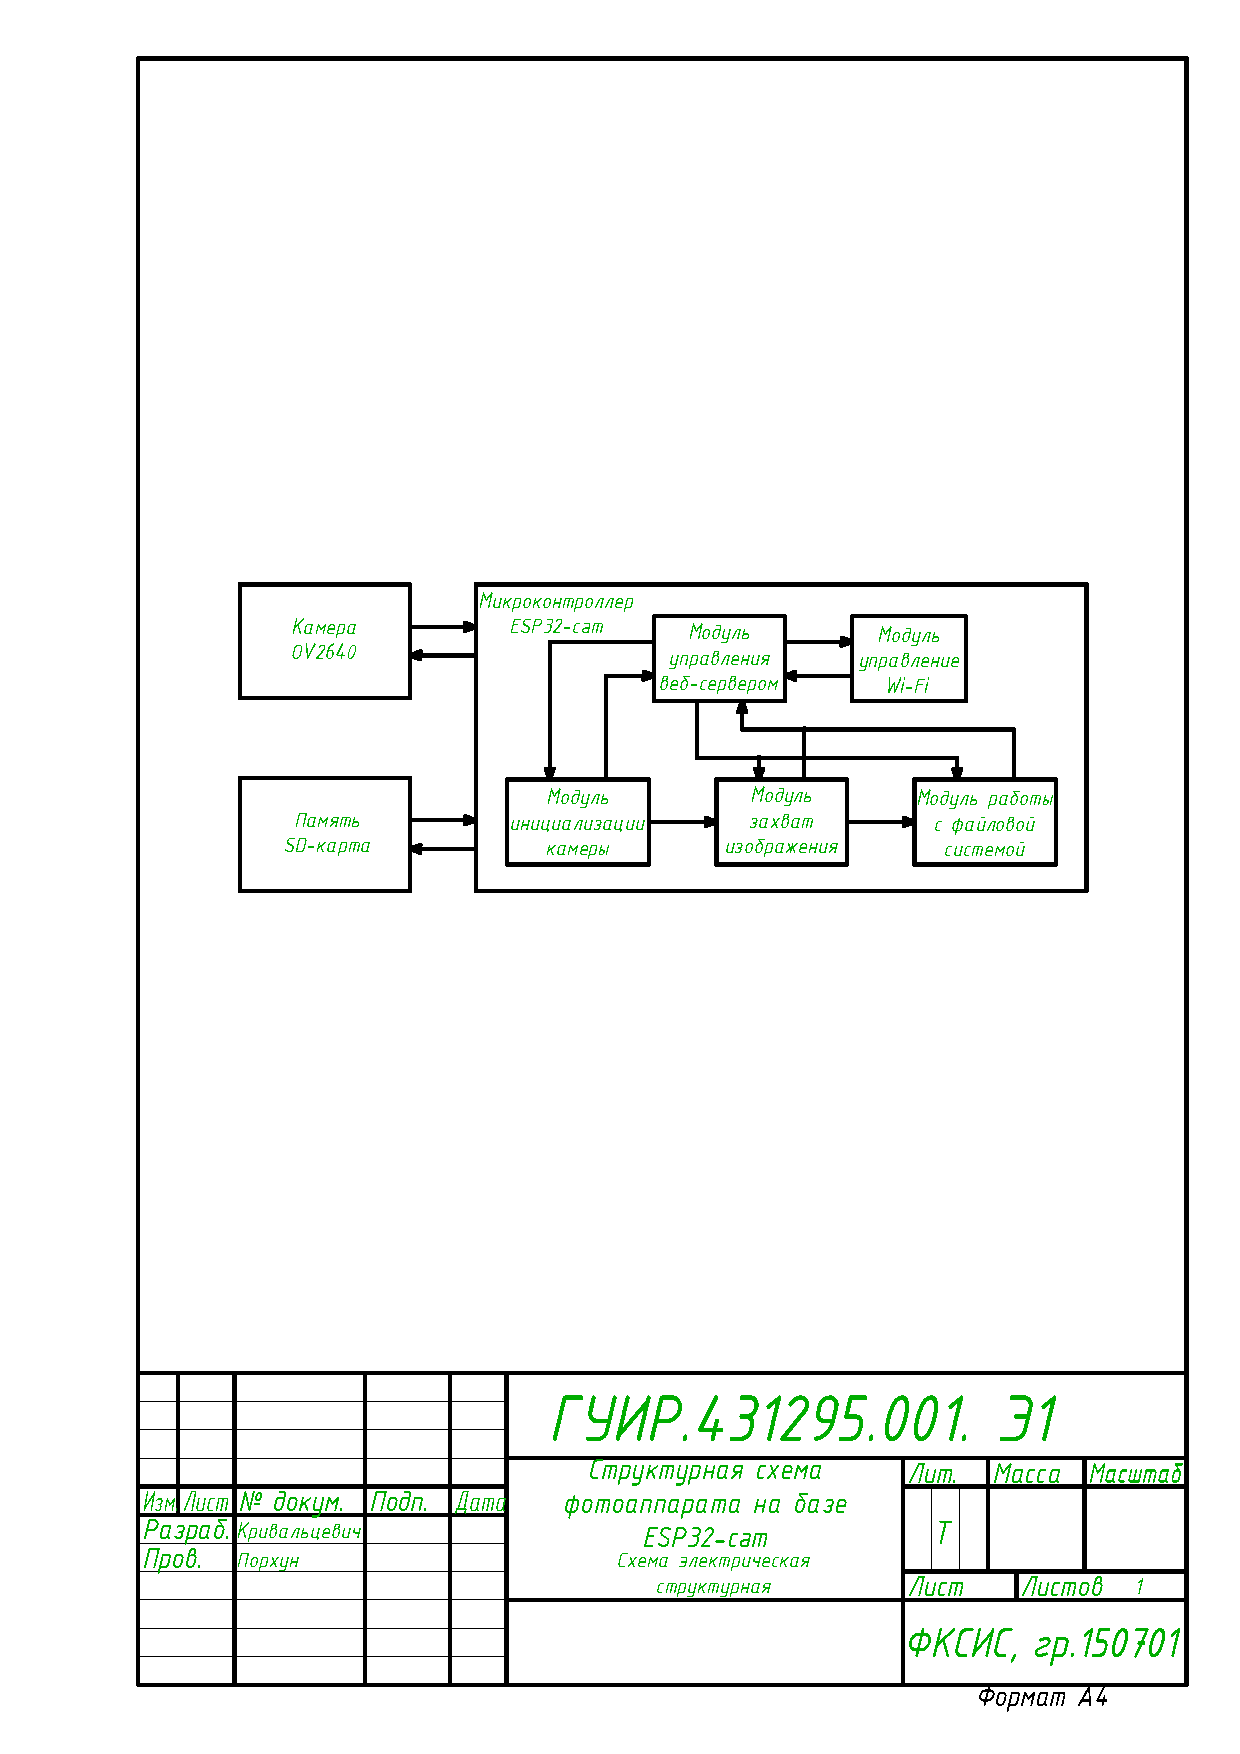
\includepdf[pages=-, pagecommand={}, fitpaper, offset=0 0]{prilA.pdf}

% Восстановление размера страницы A4
\pdfpagewidth=210mm
\pdfpageheight=297mm

\clearpage
               % Приложение А 
% Ваш основной текст
\clearpage
\phantomsection% ensures hyperref works properly
\addcontentsline{toc}{section}{\hspace*{-1em}Приложение Б (Обязательное) Пример вставки pdf}\par

\normalsize
\begin{center}
  \textbf{ПРИЛОЖЕНИЕ Б} \\
  \textbf{(Обязательное)} \\
  \textbf{Пример вставки pdf}
\end{center}

\clearpage

% Установка размера страницы A3 в альбомной ориентации
% \pdfpagewidth=420mm
% \pdfpageheight=297mm

\thispagestyle{empty} % Убрать номер страницы

% Вставка листа A3
% 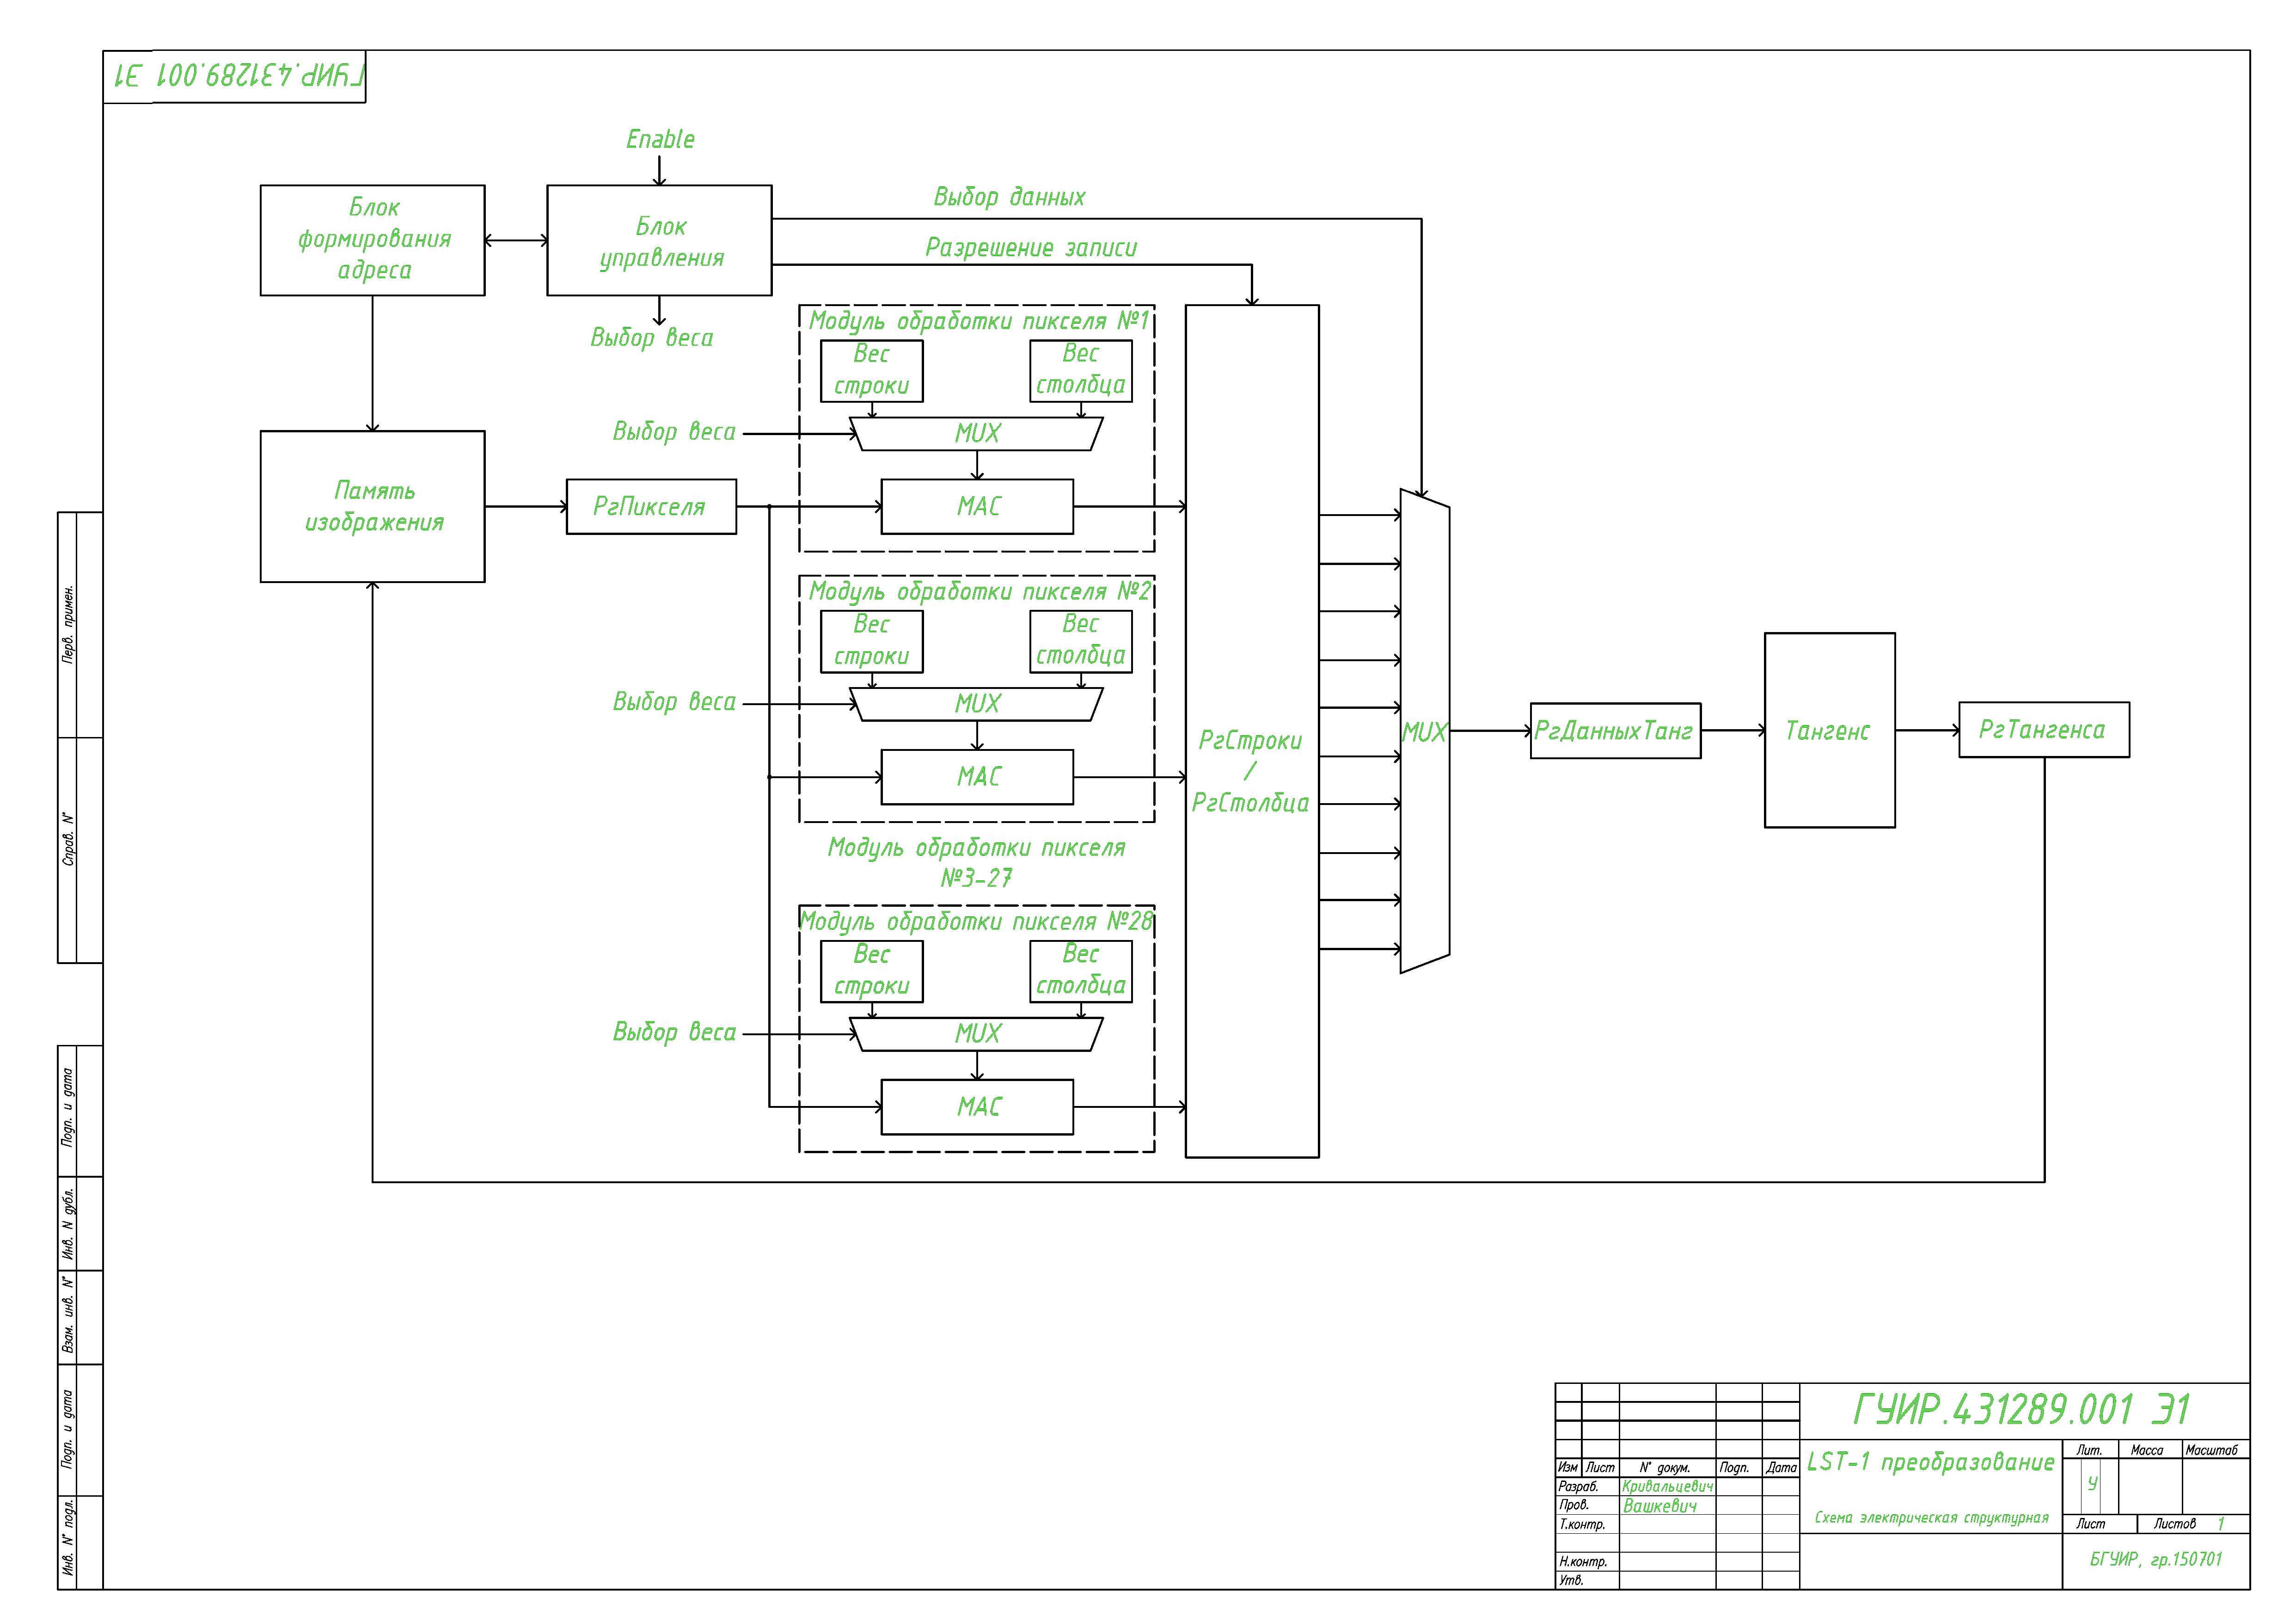
\includepdf[pages=-, pagecommand={}, fitpaper, offset=0 0]{STRUCT_LST.pdf}

% Восстановление размера страницы A4
\pdfpagewidth=210mm
\pdfpageheight=297mm

\clearpage
               % Приложение Б
% Ваш основной текст
\clearpage
\phantomsection% ensures hyperref works properly
\addcontentsline{toc}{section}{\hspace*{-1em}Приложение В (Обязательное) Схема алгоритма работы устройства}\par

\normalsize
\begin{center}
  \textbf{ПРИЛОЖЕНИЕ В} \\
  \textbf{(Обязательное)} \\
  \textbf{Схема алгоритма работы слояустройства}
\end{center}

\clearpage

% Установка размера страницы A3 в альбомной ориентации
% \pdfpagewidth=420mm
% \pdfpageheight=297mm

\thispagestyle{empty} % Убрать номер страницы

% Вставка листа A3
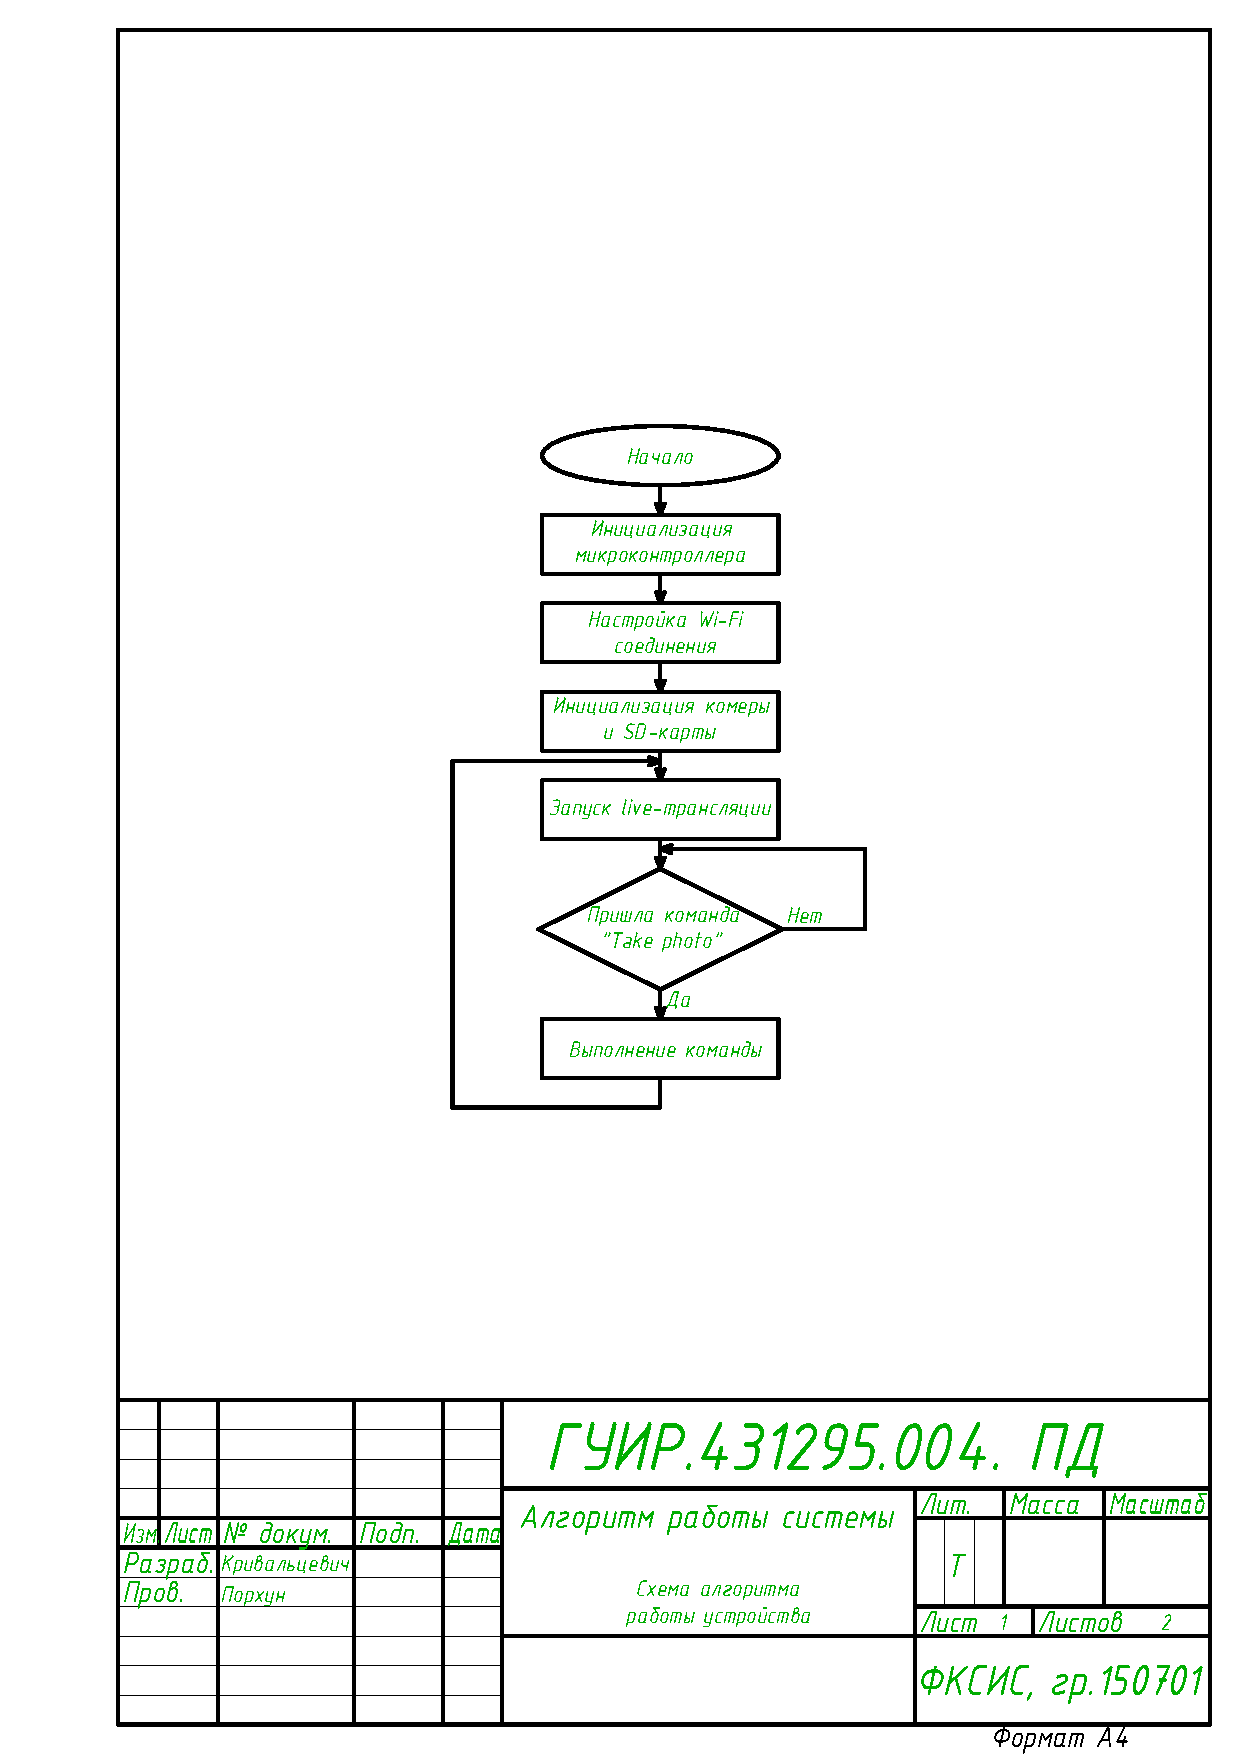
\includepdf[pages=-, pagecommand={}, fitpaper, offset=0 0]{prilC.pdf}
\thispagestyle{empty} % Убрать номер страницы
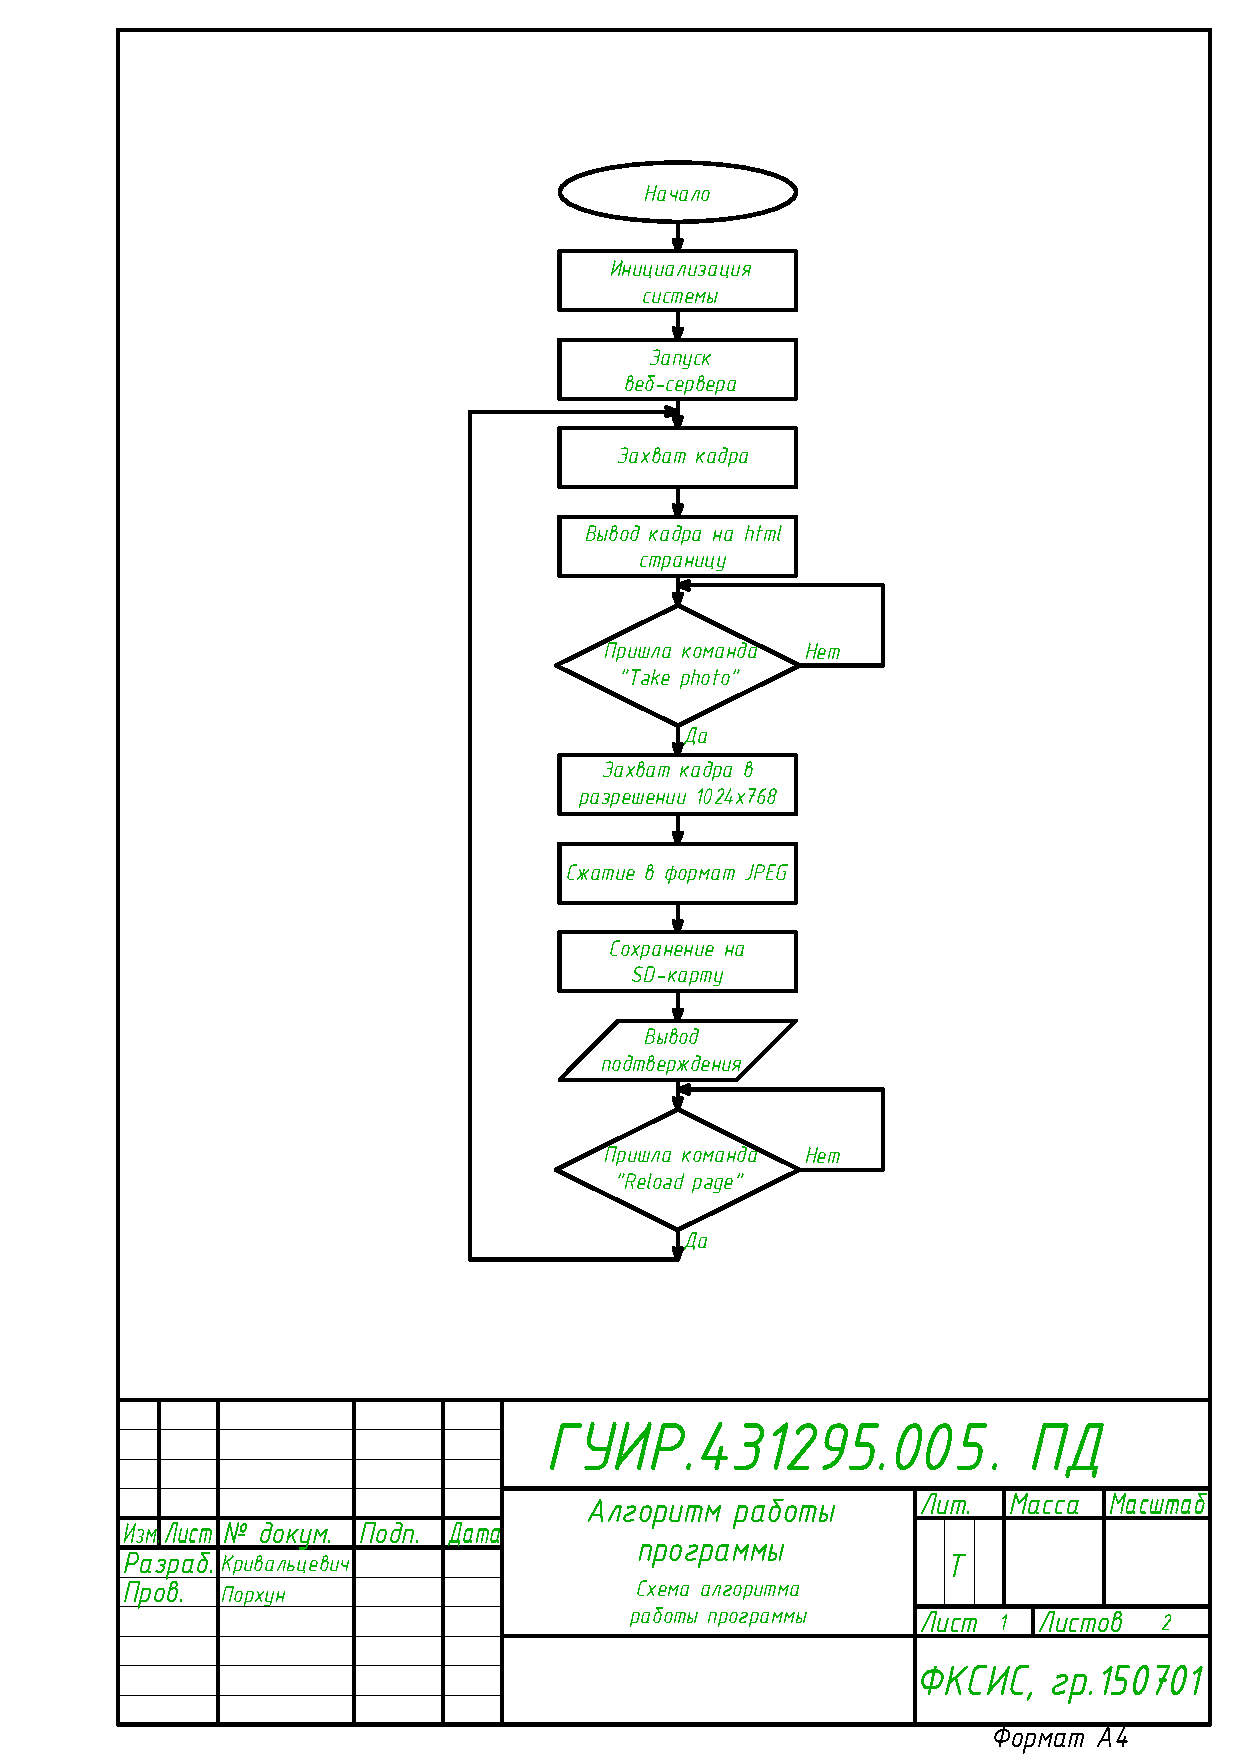
\includepdf[pages=-, pagecommand={}, fitpaper, offset=0 0]{prilC1.pdf}

% Восстановление размера страницы A4
\pdfpagewidth=210mm
\pdfpageheight=297mm
\clearpage
               % Приложение В 
\clearpage
\phantomsection% ensures hyperref works properly
\addcontentsline{toc}{section}{\hspace*{-1em}Приложение Г (Обязательное) Пример вставки pdf}\par

\normalsize
\begin{center}
  \textbf{ПРИЛОЖЕНИЕ Г} \\
  \textbf{(Обязательное)} \\
  \textbf{Пример вставки pdf}
\end{center}

\clearpage

% Установка размера страницы A3 в альбомной ориентации
% \pdfpagewidth=420mm
% \pdfpageheight=297mm

\thispagestyle{empty} % Убрать номер страницы

% Вставка листа A3
% 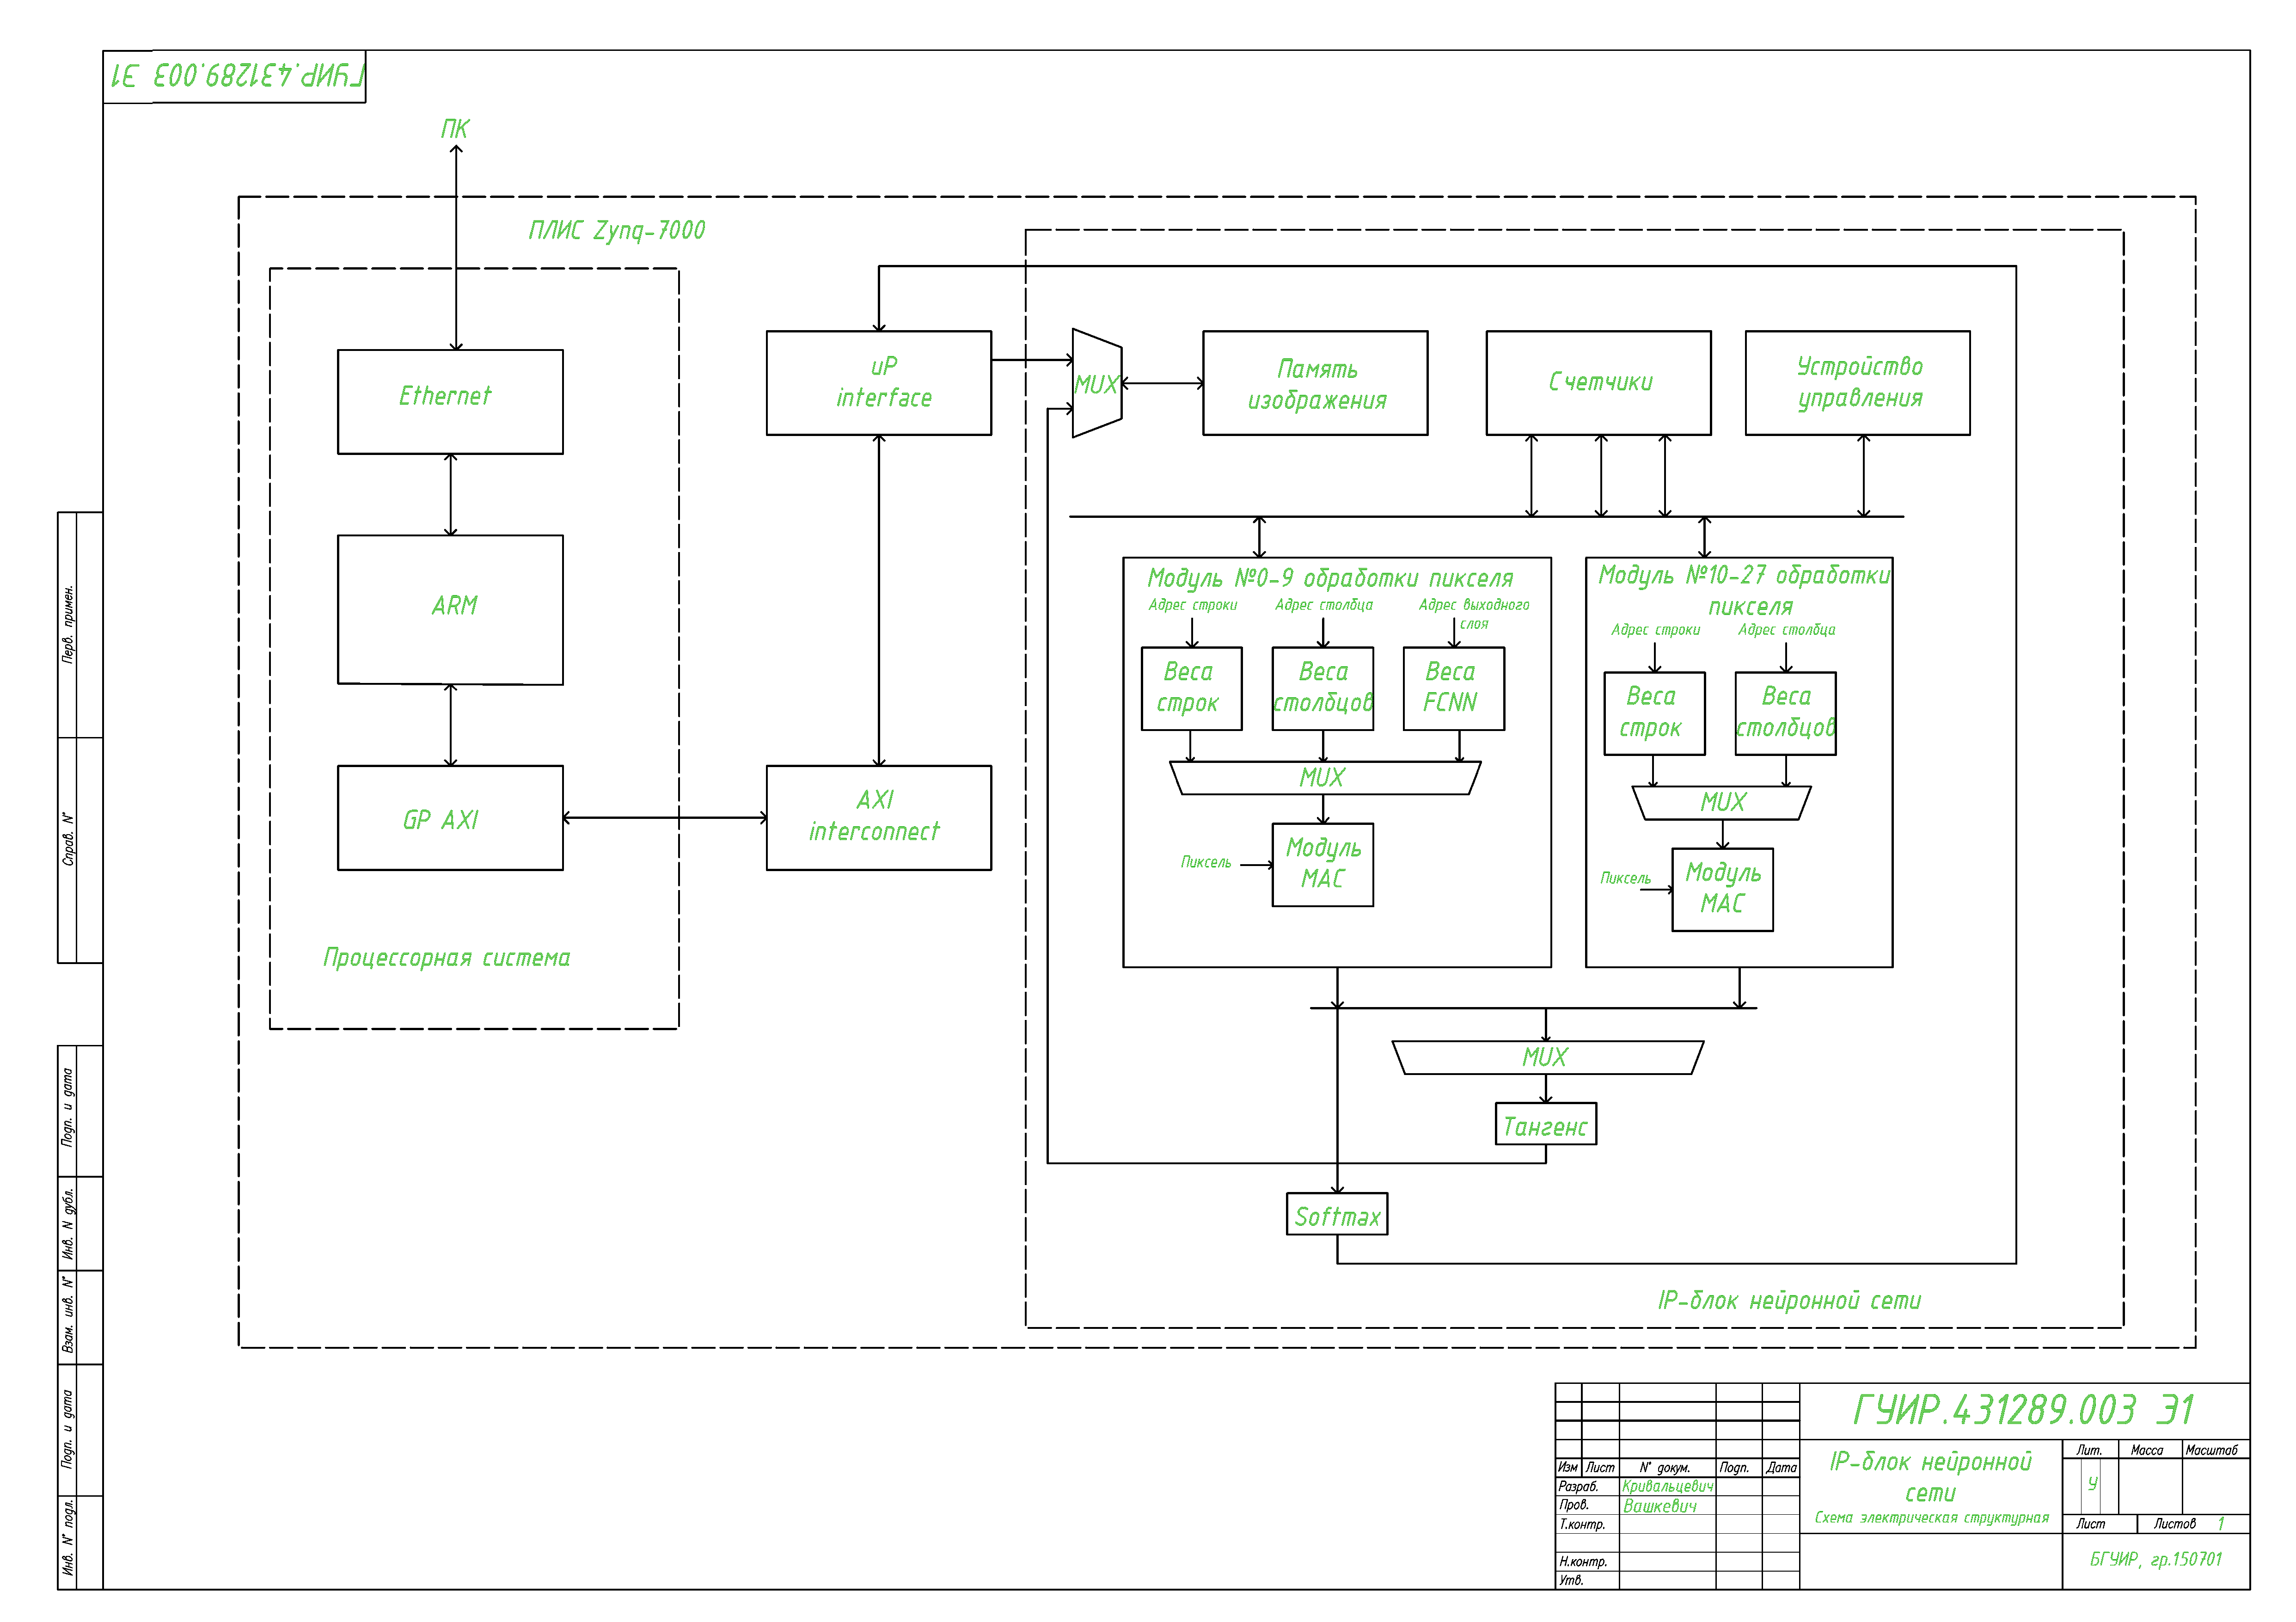
\includepdf[pages=-, pagecommand={}, fitpaper, offset=0 0]{STRUCT.pdf}
% \thispagestyle{empty} % Убрать номер страницы
% 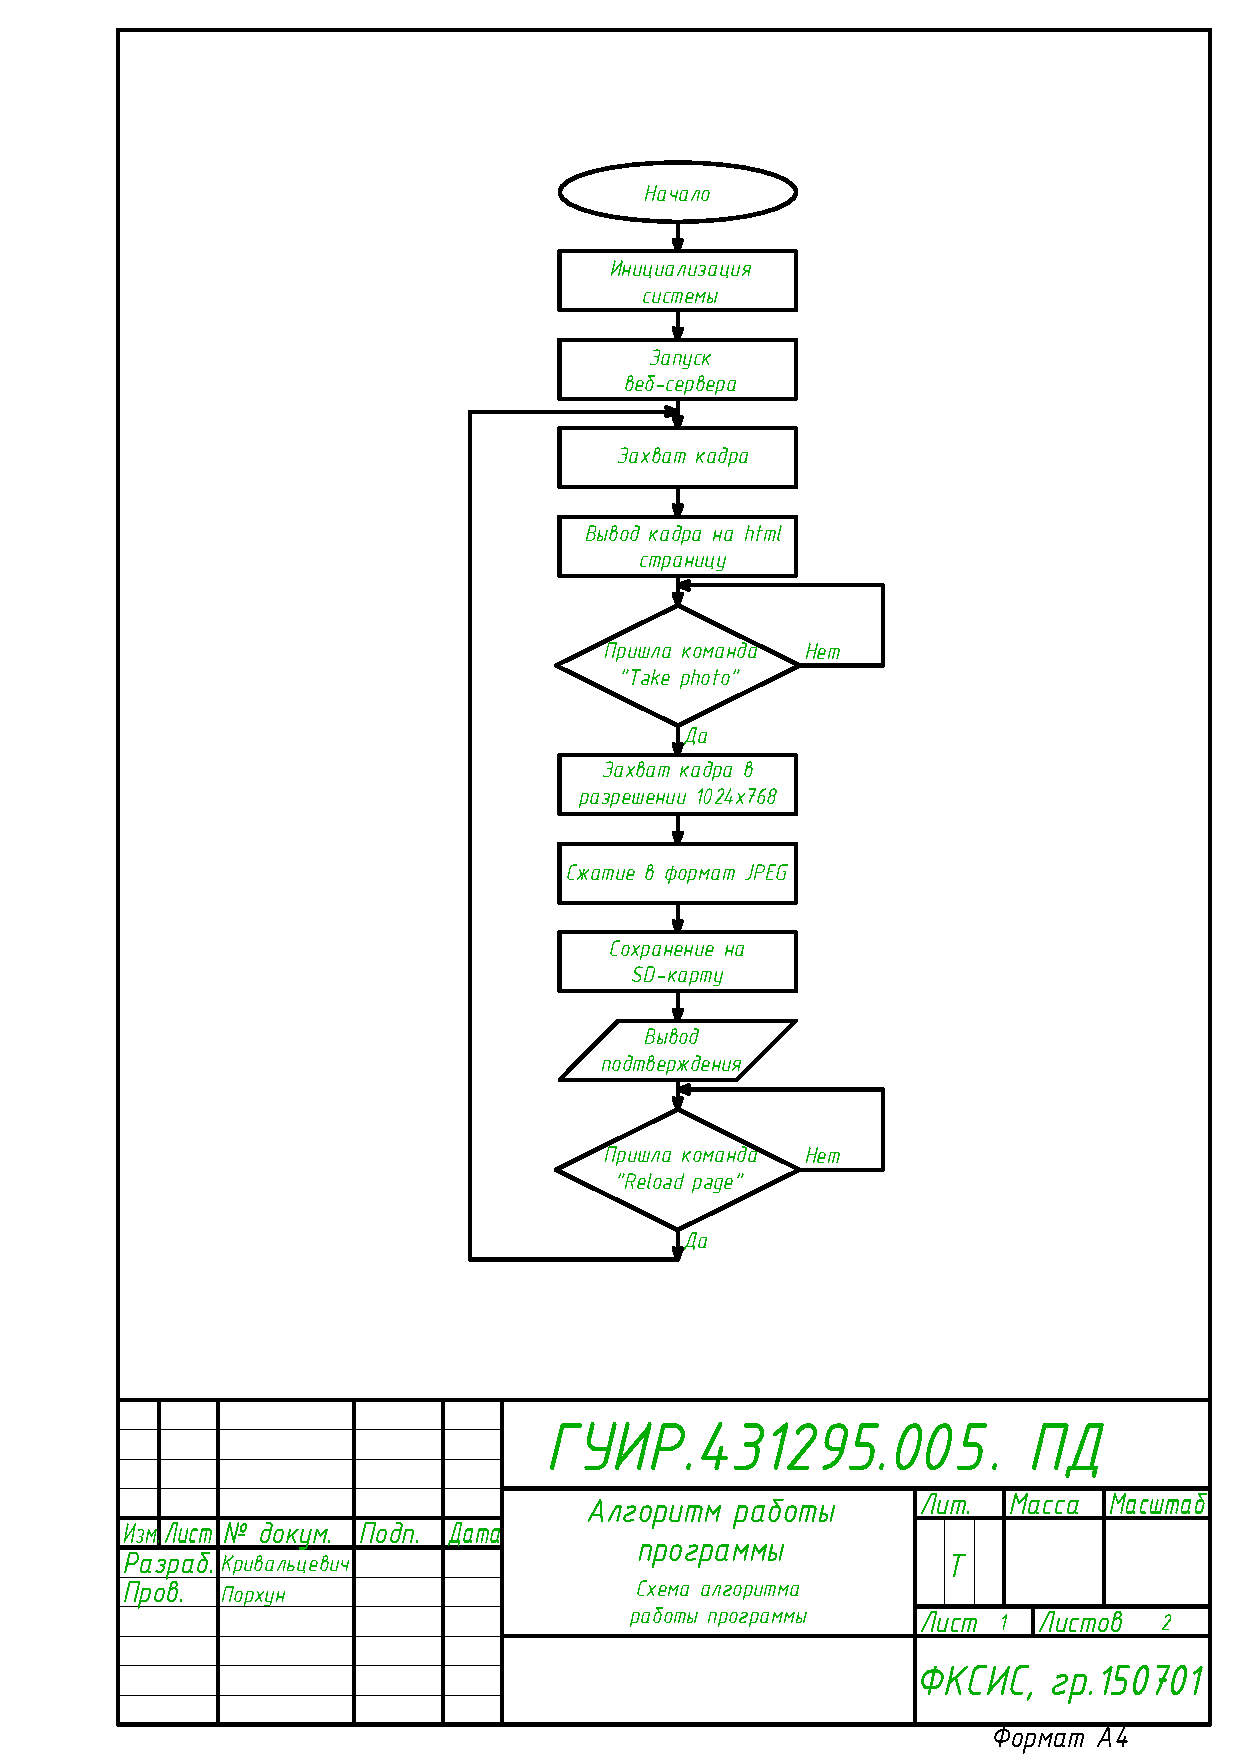
\includepdf[pages=-, pagecommand={}, fitpaper, offset=0 0]{prilC1.pdf}

% Восстановление размера страницы A4
\pdfpagewidth=210mm
\pdfpageheight=297mm

\clearpage
               % Приложение Г 
\clearpage
\phantomsection% ensures hyperref works properly
\addcontentsline{toc}{section}{\hspace*{-1em}Приложение Д (Обязательное) Пример вставки кода}\par

\normalsize
\begin{center}
  \textbf{ПРИЛОЖЕНИЕ Д} \\
  \textbf{(Обязательное)} \\
  \textbf{Пример вставки кода}
\end{center}

Пример вставки кода:

% \lstinputlisting[language=html]{C/index.html}


% Восстановление размера страницы A4
\pdfpagewidth=210mm
\pdfpageheight=297mm               % Приложение Д   

\clearpage

\thispagestyle{empty} % Убрать номер страницы

% Вставка листа A4
% 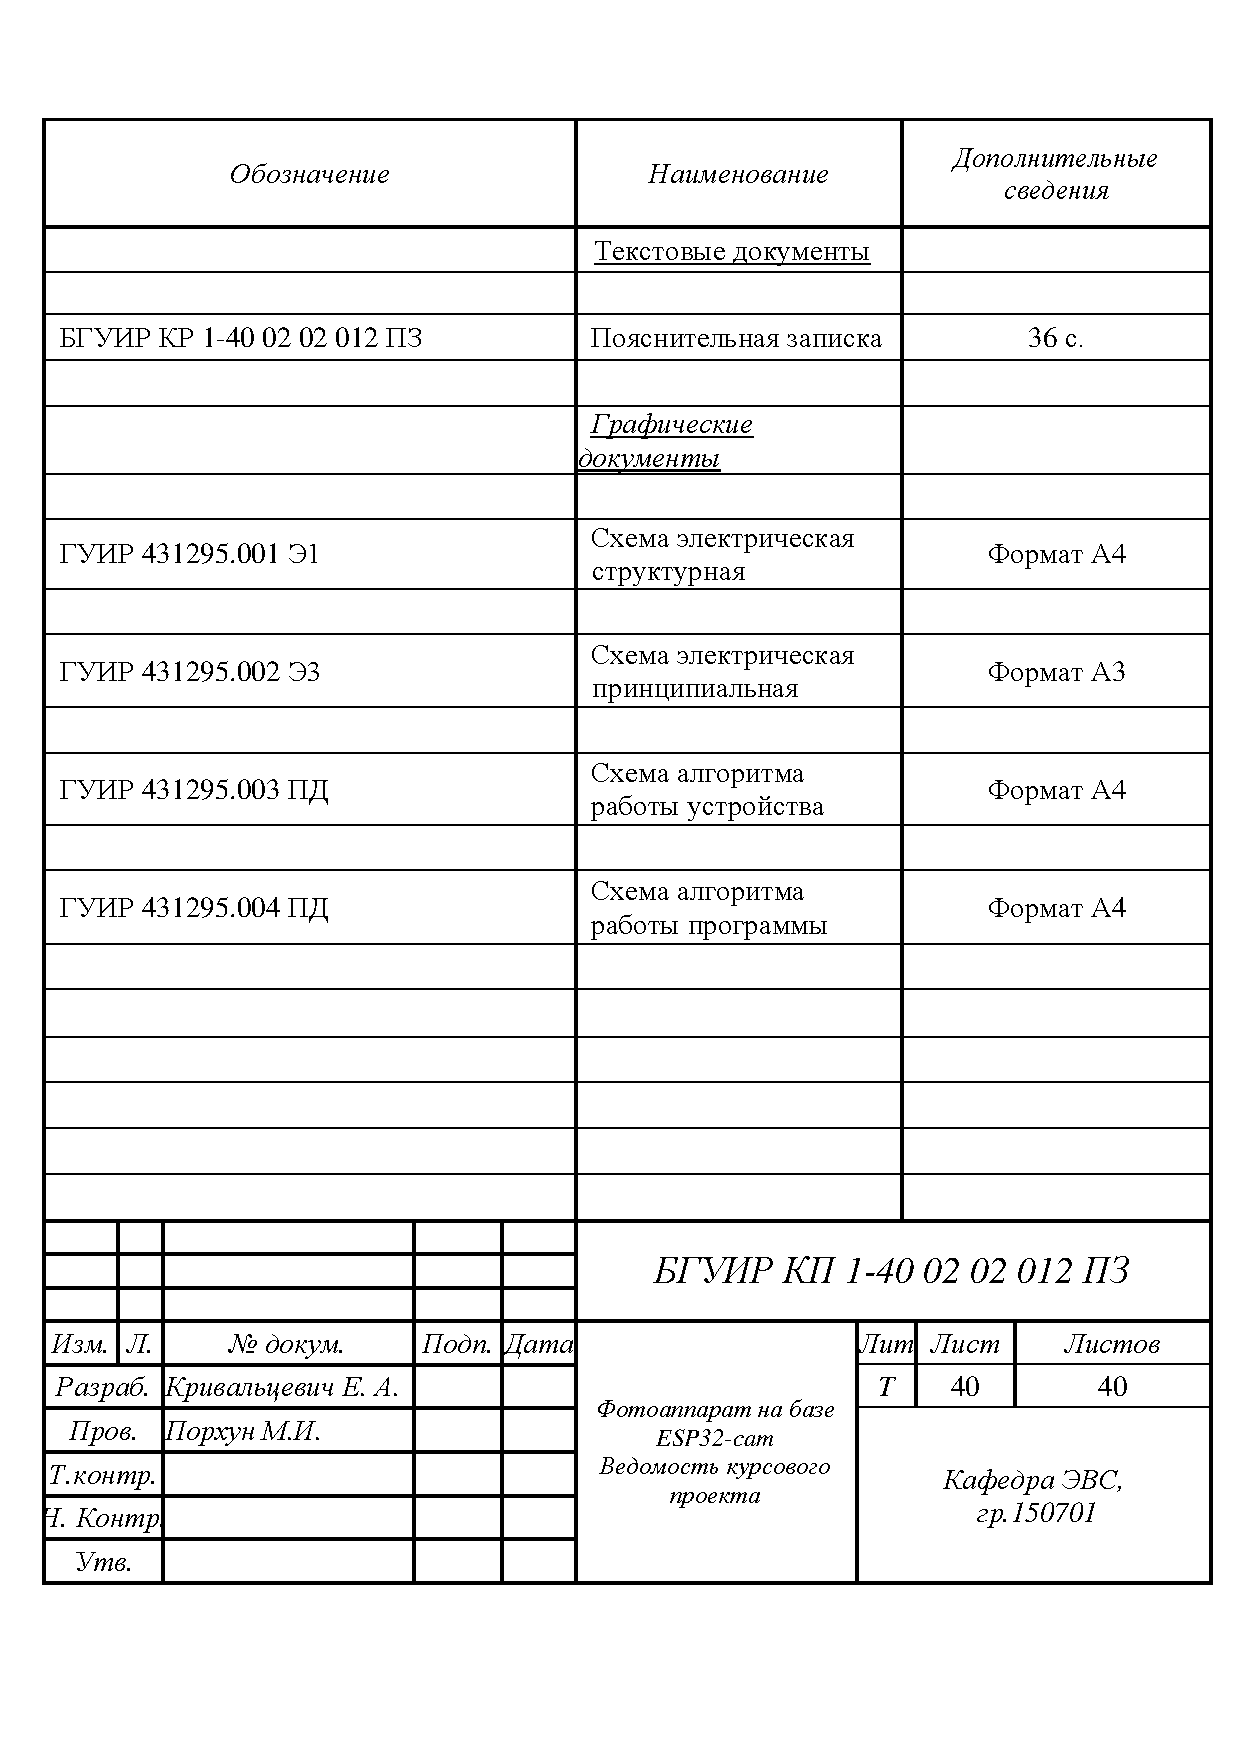
\includepdf[pages=-, pagecommand={}, fitpaper, offset=0 0]{vedoma.pdf}

% Восстановление размера страницы A4
\pdfpagewidth=210mm
\pdfpageheight=297mm

\clearpage


\end{document}
